% Options for packages loaded elsewhere
\PassOptionsToPackage{unicode}{hyperref}
\PassOptionsToPackage{hyphens}{url}
\PassOptionsToPackage{dvipsnames,svgnames,x11names}{xcolor}
%
\documentclass[
]{interact}

\usepackage{amsmath,amssymb}
\usepackage{iftex}
\ifPDFTeX
  \usepackage[T1]{fontenc}
  \usepackage[utf8]{inputenc}
  \usepackage{textcomp} % provide euro and other symbols
\else % if luatex or xetex
  \usepackage{unicode-math}
  \defaultfontfeatures{Scale=MatchLowercase}
  \defaultfontfeatures[\rmfamily]{Ligatures=TeX,Scale=1}
\fi
\usepackage{lmodern}
\ifPDFTeX\else  
    % xetex/luatex font selection
\fi
% Use upquote if available, for straight quotes in verbatim environments
\IfFileExists{upquote.sty}{\usepackage{upquote}}{}
\IfFileExists{microtype.sty}{% use microtype if available
  \usepackage[]{microtype}
  \UseMicrotypeSet[protrusion]{basicmath} % disable protrusion for tt fonts
}{}
\makeatletter
\@ifundefined{KOMAClassName}{% if non-KOMA class
  \IfFileExists{parskip.sty}{%
    \usepackage{parskip}
  }{% else
    \setlength{\parindent}{0pt}
    \setlength{\parskip}{6pt plus 2pt minus 1pt}}
}{% if KOMA class
  \KOMAoptions{parskip=half}}
\makeatother
\usepackage{xcolor}
\setlength{\emergencystretch}{3em} % prevent overfull lines
\setcounter{secnumdepth}{5}
% Make \paragraph and \subparagraph free-standing
\ifx\paragraph\undefined\else
  \let\oldparagraph\paragraph
  \renewcommand{\paragraph}[1]{\oldparagraph{#1}\mbox{}}
\fi
\ifx\subparagraph\undefined\else
  \let\oldsubparagraph\subparagraph
  \renewcommand{\subparagraph}[1]{\oldsubparagraph{#1}\mbox{}}
\fi

\usepackage{color}
\usepackage{fancyvrb}
\newcommand{\VerbBar}{|}
\newcommand{\VERB}{\Verb[commandchars=\\\{\}]}
\DefineVerbatimEnvironment{Highlighting}{Verbatim}{commandchars=\\\{\}}
% Add ',fontsize=\small' for more characters per line
\usepackage{framed}
\definecolor{shadecolor}{RGB}{241,243,245}
\newenvironment{Shaded}{\begin{snugshade}}{\end{snugshade}}
\newcommand{\AlertTok}[1]{\textcolor[rgb]{0.68,0.00,0.00}{#1}}
\newcommand{\AnnotationTok}[1]{\textcolor[rgb]{0.37,0.37,0.37}{#1}}
\newcommand{\AttributeTok}[1]{\textcolor[rgb]{0.40,0.45,0.13}{#1}}
\newcommand{\BaseNTok}[1]{\textcolor[rgb]{0.68,0.00,0.00}{#1}}
\newcommand{\BuiltInTok}[1]{\textcolor[rgb]{0.00,0.23,0.31}{#1}}
\newcommand{\CharTok}[1]{\textcolor[rgb]{0.13,0.47,0.30}{#1}}
\newcommand{\CommentTok}[1]{\textcolor[rgb]{0.37,0.37,0.37}{#1}}
\newcommand{\CommentVarTok}[1]{\textcolor[rgb]{0.37,0.37,0.37}{\textit{#1}}}
\newcommand{\ConstantTok}[1]{\textcolor[rgb]{0.56,0.35,0.01}{#1}}
\newcommand{\ControlFlowTok}[1]{\textcolor[rgb]{0.00,0.23,0.31}{#1}}
\newcommand{\DataTypeTok}[1]{\textcolor[rgb]{0.68,0.00,0.00}{#1}}
\newcommand{\DecValTok}[1]{\textcolor[rgb]{0.68,0.00,0.00}{#1}}
\newcommand{\DocumentationTok}[1]{\textcolor[rgb]{0.37,0.37,0.37}{\textit{#1}}}
\newcommand{\ErrorTok}[1]{\textcolor[rgb]{0.68,0.00,0.00}{#1}}
\newcommand{\ExtensionTok}[1]{\textcolor[rgb]{0.00,0.23,0.31}{#1}}
\newcommand{\FloatTok}[1]{\textcolor[rgb]{0.68,0.00,0.00}{#1}}
\newcommand{\FunctionTok}[1]{\textcolor[rgb]{0.28,0.35,0.67}{#1}}
\newcommand{\ImportTok}[1]{\textcolor[rgb]{0.00,0.46,0.62}{#1}}
\newcommand{\InformationTok}[1]{\textcolor[rgb]{0.37,0.37,0.37}{#1}}
\newcommand{\KeywordTok}[1]{\textcolor[rgb]{0.00,0.23,0.31}{#1}}
\newcommand{\NormalTok}[1]{\textcolor[rgb]{0.00,0.23,0.31}{#1}}
\newcommand{\OperatorTok}[1]{\textcolor[rgb]{0.37,0.37,0.37}{#1}}
\newcommand{\OtherTok}[1]{\textcolor[rgb]{0.00,0.23,0.31}{#1}}
\newcommand{\PreprocessorTok}[1]{\textcolor[rgb]{0.68,0.00,0.00}{#1}}
\newcommand{\RegionMarkerTok}[1]{\textcolor[rgb]{0.00,0.23,0.31}{#1}}
\newcommand{\SpecialCharTok}[1]{\textcolor[rgb]{0.37,0.37,0.37}{#1}}
\newcommand{\SpecialStringTok}[1]{\textcolor[rgb]{0.13,0.47,0.30}{#1}}
\newcommand{\StringTok}[1]{\textcolor[rgb]{0.13,0.47,0.30}{#1}}
\newcommand{\VariableTok}[1]{\textcolor[rgb]{0.07,0.07,0.07}{#1}}
\newcommand{\VerbatimStringTok}[1]{\textcolor[rgb]{0.13,0.47,0.30}{#1}}
\newcommand{\WarningTok}[1]{\textcolor[rgb]{0.37,0.37,0.37}{\textit{#1}}}

\providecommand{\tightlist}{%
  \setlength{\itemsep}{0pt}\setlength{\parskip}{0pt}}\usepackage{longtable,booktabs,array}
\usepackage{calc} % for calculating minipage widths
% Correct order of tables after \paragraph or \subparagraph
\usepackage{etoolbox}
\makeatletter
\patchcmd\longtable{\par}{\if@noskipsec\mbox{}\fi\par}{}{}
\makeatother
% Allow footnotes in longtable head/foot
\IfFileExists{footnotehyper.sty}{\usepackage{footnotehyper}}{\usepackage{footnote}}
\makesavenoteenv{longtable}
\usepackage{graphicx}
\makeatletter
\def\maxwidth{\ifdim\Gin@nat@width>\linewidth\linewidth\else\Gin@nat@width\fi}
\def\maxheight{\ifdim\Gin@nat@height>\textheight\textheight\else\Gin@nat@height\fi}
\makeatother
% Scale images if necessary, so that they will not overflow the page
% margins by default, and it is still possible to overwrite the defaults
% using explicit options in \includegraphics[width, height, ...]{}
\setkeys{Gin}{width=\maxwidth,height=\maxheight,keepaspectratio}
% Set default figure placement to htbp
\makeatletter
\def\fps@figure{htbp}
\makeatother
\newlength{\cslhangindent}
\setlength{\cslhangindent}{1.5em}
\newlength{\csllabelwidth}
\setlength{\csllabelwidth}{3em}
\newlength{\cslentryspacingunit} % times entry-spacing
\setlength{\cslentryspacingunit}{\parskip}
\newenvironment{CSLReferences}[2] % #1 hanging-ident, #2 entry spacing
 {% don't indent paragraphs
  \setlength{\parindent}{0pt}
  % turn on hanging indent if param 1 is 1
  \ifodd #1
  \let\oldpar\par
  \def\par{\hangindent=\cslhangindent\oldpar}
  \fi
  % set entry spacing
  \setlength{\parskip}{#2\cslentryspacingunit}
 }%
 {}
\usepackage{calc}
\newcommand{\CSLBlock}[1]{#1\hfill\break}
\newcommand{\CSLLeftMargin}[1]{\parbox[t]{\csllabelwidth}{#1}}
\newcommand{\CSLRightInline}[1]{\parbox[t]{\linewidth - \csllabelwidth}{#1}\break}
\newcommand{\CSLIndent}[1]{\hspace{\cslhangindent}#1}

\usepackage{scrlayer-scrpage}
\rohead{Preprint: Not Peer Reviewed}
\usepackage{orcidlink}
\makeatletter
\makeatother
\makeatletter
\makeatother
\makeatletter
\@ifpackageloaded{caption}{}{\usepackage{caption}}
\AtBeginDocument{%
\ifdefined\contentsname
  \renewcommand*\contentsname{Table of contents}
\else
  \newcommand\contentsname{Table of contents}
\fi
\ifdefined\listfigurename
  \renewcommand*\listfigurename{List of Figures}
\else
  \newcommand\listfigurename{List of Figures}
\fi
\ifdefined\listtablename
  \renewcommand*\listtablename{List of Tables}
\else
  \newcommand\listtablename{List of Tables}
\fi
\ifdefined\figurename
  \renewcommand*\figurename{Figure}
\else
  \newcommand\figurename{Figure}
\fi
\ifdefined\tablename
  \renewcommand*\tablename{Table}
\else
  \newcommand\tablename{Table}
\fi
}
\@ifpackageloaded{float}{}{\usepackage{float}}
\floatstyle{ruled}
\@ifundefined{c@chapter}{\newfloat{codelisting}{h}{lop}}{\newfloat{codelisting}{h}{lop}[chapter]}
\floatname{codelisting}{Listing}
\newcommand*\listoflistings{\listof{codelisting}{List of Listings}}
\makeatother
\makeatletter
\@ifpackageloaded{caption}{}{\usepackage{caption}}
\@ifpackageloaded{subcaption}{}{\usepackage{subcaption}}
\makeatother
\makeatletter
\@ifpackageloaded{tcolorbox}{}{\usepackage[skins,breakable]{tcolorbox}}
\makeatother
\makeatletter
\@ifundefined{shadecolor}{\definecolor{shadecolor}{rgb}{.97, .97, .97}}
\makeatother
\makeatletter
\makeatother
\makeatletter
\makeatother
\ifLuaTeX
  \usepackage{selnolig}  % disable illegal ligatures
\fi
\IfFileExists{bookmark.sty}{\usepackage{bookmark}}{\usepackage{hyperref}}
\IfFileExists{xurl.sty}{\usepackage{xurl}}{} % add URL line breaks if available
\urlstyle{same} % disable monospaced font for URLs
\hypersetup{
  pdftitle={Exploring Equivalence Testing with the Updated TOSTER R Package},
  pdfauthor={Aaron R. Caldwell},
  pdfkeywords={statistics, bootstrap, minimal effects test, NHST, TOST,
R},
  colorlinks=true,
  linkcolor={blue},
  filecolor={Maroon},
  citecolor={Blue},
  urlcolor={Blue},
  pdfcreator={LaTeX via pandoc}}

\title{Exploring Equivalence Testing with the Updated TOSTER R Package}
\author{Aaron R.
Caldwell$\textsuperscript{1}$~\orcidlink{0000-0002-4541-6283}}

\thanks{CONTACT: Aaron R.
Caldwell. Email: \href{mailto:caldwellaaron@uams.edu}{\nolinkurl{caldwellaaron@uams.edu}}. }
\begin{document}
\captionsetup{labelsep=space}
\maketitle
\textsuperscript{1} Office of Community Health and Research, Fay W.
Boozman College of Public Health, University of Arkansas for Medical
Sciences Northwest, Springdale, AR, USA
\begin{abstract}
Equivalence testing is arguably under utilized by experimental
researchers. Due to limited software support for such analyses, and
little education on the topic in graduate programs, the utilization of
equivalence testings still appares to be low. One option for equivalence
testing is the use of two one-sided tests (TOST). The TOSTER R package
and jamovi module, originally developed by Daniel Lakens in 2017, was
created to make TOST more accessible to the average researcher. In the
past four years, I have made significant changes to the TOSTER package
in order to increase its accessibility and provide more robust analysis
options for researchers. In this paper, I will detail the changes to the
package and highlight new analysis options that will make TOST easier
for the average quantitative researcher.
\end{abstract}
\begin{keywords}
\def\sep{;\ }
statistics, bootstrap, minimal effects test, NHST, TOST, R\sep 
statistics, bootstrap, minimal effects test, NHST, TOST, R
\end{keywords}
\ifdefined\Shaded\renewenvironment{Shaded}{\begin{tcolorbox}[interior hidden, boxrule=0pt, borderline west={3pt}{0pt}{shadecolor}, enhanced, frame hidden, breakable, sharp corners]}{\end{tcolorbox}}\fi

\hypertarget{introduction}{%
\section{Introduction}\label{introduction}}

Researchers often erroneously declare that no statistical effect exists
based on a single ``non-significant'' p-value
(\protect\hyperlink{ref-blandaltman95}{Altman and Bland 1995}). In many
of these cases, the data may corroborate the researcher's claim, but the
interpretation of a null hypothesis significance test (NHST), wherein
the lack of significance is considered evidence of ``no effect'', is
nonetheless incorrect. In order to statistically test whether there is
no effect, researchers could use equivalence testing. Equivalence
testing is typically used when the goal of a statistical test is to
demonstrate that the difference between two conditions is too small to
be meaningful. For example, if a researcher wanted to test whether a new
drug was no worse than a standard drug, the null hypothesis would be
that the new drug is worse than the standard drug by more than a
meaningful amount, and the alternative hypothesis would be that the
difference between the two drugs is small enough to be meaningless. A
very simple equivalence testing approach is the use of two one-sided
tests (TOST) (\protect\hyperlink{ref-schuirmann1987}{Schuirmann 1987}).

The TOST procedure is a statistical test of whether a parameter (e.g.,
mean difference) is within a specified interval. The TOST procedure can
be used to test the equivalence of two means, two proportions, two
regression coefficients, and even two variances. For a test of mean
difference, an upper (\(\Delta_U\)) and lower (\(\Delta_L\)) equivalence
bound is specified based on the smallest effect size of interest
(SESOI). If the TOST is below the pre-specified alpha level, then the
effect can be considered close enough to zero to be practically
equivalent (\protect\hyperlink{ref-lakens_ori}{Lakens 2017}).

Both the complaints about erroneous conclusions regarding equivalence
(\protect\hyperlink{ref-blandaltman95}{Altman and Bland 1995}) and
proposed statistical solutions
(\protect\hyperlink{ref-schuirmann1987}{Schuirmann 1987}) have existed
for decades now. Yet, the problem appears to persist in many applied
disciplines. I believe the continued dissonance is due to a general lack
of education on equivalence testing and a struggle for many applied
researchers to implement equivalence testing. In my experience, most
researchers have received some degree of statistical training in their
doctoral or master's studies, but it is rare that any have idea of how
to implement equivalence testing. This may be caused by most statistical
software defaulting to a null hypothesis of zero, or even completely
lacking an ability to change the null hypothesis. Therefore, I feel the
continued development of educational content on TOST, and software to
help with such analyses, is be beneficial to many quantitative
researchers.

The TOSTER R package\footnote{All updates to the package can be found on
  the package's website \url{https://aaroncaldwell.us/TOSTERpkg}.} was
originally developed in by Lakens
(\protect\hyperlink{ref-lakens_ori}{2017}) to introduce experimental
psychologists to the concept of equivalence testing and provide an
easy-to-use implementation in R. In the years since that publication, I
have made a significant update to the package in order to improve the
user interface and expand the tools available within the package. An
experienced R programmer may have no problem performing equivalence
testing within R, but beginners may struggle with both writing the code
and interpreting the output. The TOSTER R package is made for those with
at least a beginner's knowledge of R. However, others may lack any
knowledge of how to use R. If you fall into that category, I would
suggest using jamovi, an open-source statistical software, that has a
TOSTER module to perform some equivalence/TOST analyses. Not all the
features listed in this manuscript are available in the jamovi module,
but it is a good starting point for most researchers without statistical
programming experience.

In this manuscript, I will detail the updates to the TOSTER package, and
give some basic guidance on how to use this package for equivalence
testing. This is meant to just be an introduction on \emph{how} to
perform such analyses, and provide a little bit of context for when such
analyses are appropriate. For a greater introduction to the concept of
equivalence testing, I would suggest reading other methodological
tutorials (\protect\hyperlink{ref-lakens_ori}{Lakens 2017};
\protect\hyperlink{ref-lakens2018equivalence}{Lakens, Scheel, and Isager
2018}; \protect\hyperlink{ref-lakens2020improving}{Lakens et al. 2020};
\protect\hyperlink{ref-mazzolari2022myths}{Mazzolari et al. 2022}).

\hypertarget{tost-with-t-tests}{%
\section{TOST with t-tests}\label{tost-with-t-tests}}

In an effort to make TOSTER more informative and easier to use, the
\texttt{t\_TOST} and \texttt{simple\_htest} fucntions were created. The
\texttt{t\_TOST} function operates very similarly to base R's
\texttt{t.test} function, but performs 3 t-tests (one two-tailed and two
one-tailed tests). In addition, this function has a generic method where
two vectors can be supplied or a formula can be given
(e.g.,\texttt{y\ \textasciitilde{}\ group}). This function also makes it
easier to switch between types of t-tests. All three types (two sample,
one sample, and paired samples) can be performed/calculated from the
same function. Moreover, the output from this function is verbose, and
should make the decisions derived from the function more informative and
user-friendly. Also, \texttt{t\_TOST} is not limited to equivalence
tests. Minimal effects testing (MET) is possible. MET is useful for
situations where the hypothesis is about a minimal effect and the
\emph{null hypothesis is equivalence} (see Figure 1)
(\protect\hyperlink{ref-mazzolari2022myths}{Mazzolari et al. 2022}).

On the other hand, the \texttt{simple\_htest} function, which also
allows for equivalence testing, provides output that exactly matches the
base \texttt{t.test} function. Instead of providing the results of 3
tests it only provides the result of 1 test that is specified by the
user. Options include a two-tailed test, one-tailed test (greater or
less), an equivalence test, or a minimal effects test. Unlike the
\texttt{t\_TOST} function, the \texttt{simple\_htest} function is
succinct in its output which may be desirable to some users.

\begin{figure}[H]

{\centering 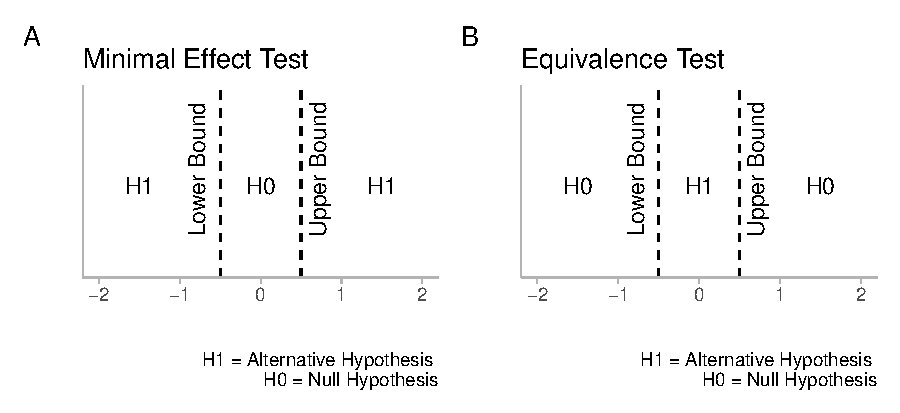
\includegraphics{avocado-quarto_files/figure-pdf/hypplot-1.pdf}

}

\caption{Type of Hypothesis}

\end{figure}

In these examples of \texttt{t\_TOST}, we will use the \texttt{bugs}
data from the \texttt{jmv} R package and the \texttt{sleep} data.

\begin{Shaded}
\begin{Highlighting}[]
\FunctionTok{data}\NormalTok{(}\StringTok{\textquotesingle{}sleep\textquotesingle{}}\NormalTok{)}
\FunctionTok{library}\NormalTok{(jmv)}
\FunctionTok{data}\NormalTok{(}\StringTok{\textquotesingle{}bugs\textquotesingle{}}\NormalTok{)}
\end{Highlighting}
\end{Shaded}

\hypertarget{independent-groups}{%
\subsection{Independent Groups}\label{independent-groups}}

For this example, we will use the sleep data. In this data, there is a
\texttt{group} variable and an outcome \texttt{extra}.

\begin{Shaded}
\begin{Highlighting}[]
\FunctionTok{head}\NormalTok{(sleep,}\DecValTok{2}\NormalTok{)}
\end{Highlighting}
\end{Shaded}

\begin{verbatim}
  extra group ID
1   0.7     1  1
2  -1.6     1  2
\end{verbatim}

We will assume the data are independent (in reality this is paired
data), and that we have equivalence bounds of +/- 0.5 units of
\texttt{extra}. All we need to do is provide the \texttt{formula},
\texttt{data}, and \texttt{eqb} arguments for the function to run
appropriately. In addition, we can set the \texttt{var.equal} argument
(to assume equal variance), and the \texttt{paired} argument (sets if
the data is paired or not). Both are logical indicators that can be set
to TRUE or FALSE. The \texttt{alpha} is automatically set to 0.05 but
this can also be adjusted by the user depending on the desired
alpha-level\footnote{I strongly recommend users ``justify their alpha''
  (\protect\hyperlink{ref-jya1}{Lakens, D., et al 2018};
  \protect\hyperlink{ref-jya2}{Maier and Lakens 2022}), and the
  justification process can be aided by my other R package
  \href{https://aaroncaldwell.us/Superpower}{Superpower}}.

Standardize mean differences (SMDs) are provided in the output from
\texttt{t\_TOST} s (e.g., Cohen's d). The Hedges's corrected SMD
(\protect\hyperlink{ref-hedges_bias}{Hedges 1981}) is automatically
calculated, but this can be overridden with the
\texttt{bias\_correction} argument\footnote{Glass's delta can also be
  produced in the output by using the \texttt{glass} argument}. In
previous versions of this package, the equivalence bounds could be set
by the SMD (e.g., equivalence bound of 0.5 SD), but this is an erroneous
approach since the bound would be dependent upon the \emph{sample}
variance. However, users can opt for such an analysis by setting
\texttt{eqbound\_type} to SMD, which will produce a noticeable warning
to the R console.

The \texttt{hypothesis} argument is automatically set to ``EQU'' for
equivalence, but if a minimal effect is of interest then ``MET'' can be
supplied.

\begin{Shaded}
\begin{Highlighting}[]
\CommentTok{\# Formula Interface}
\NormalTok{res1 }\OtherTok{=} \FunctionTok{t\_TOST}\NormalTok{(}\AttributeTok{formula =}\NormalTok{ extra }\SpecialCharTok{\textasciitilde{}}\NormalTok{ group, }\AttributeTok{data =}\NormalTok{ sleep, }
              \AttributeTok{eqb =}\NormalTok{ .}\DecValTok{5}\NormalTok{, }\AttributeTok{smd\_ci =} \StringTok{"t"}\NormalTok{)}
\CommentTok{\# x \& y Interface}
\NormalTok{res1a }\OtherTok{=} \FunctionTok{t\_TOST}\NormalTok{(}\AttributeTok{x =} \FunctionTok{subset}\NormalTok{(sleep,group}\SpecialCharTok{==}\DecValTok{1}\NormalTok{)}\SpecialCharTok{$}\NormalTok{extra,}
               \AttributeTok{y =} \FunctionTok{subset}\NormalTok{(sleep,group}\SpecialCharTok{==}\DecValTok{2}\NormalTok{)}\SpecialCharTok{$}\NormalTok{extra, }\AttributeTok{eqb =}\NormalTok{.}\DecValTok{5}\NormalTok{)}
\end{Highlighting}
\end{Shaded}

Users can also perform the same analysis with \texttt{simple\_htest} but
the SMD will not be calculated.

\begin{Shaded}
\begin{Highlighting}[]
\NormalTok{res\_1\_simple }\OtherTok{=} \FunctionTok{simple\_htest}\NormalTok{(}\AttributeTok{formula =}\NormalTok{ extra }\SpecialCharTok{\textasciitilde{}}\NormalTok{ group, }
                            \AttributeTok{data =}\NormalTok{ sleep, }
                            \AttributeTok{alternative =} \StringTok{"equivalence"}\NormalTok{, }\CommentTok{\# set hypothesis test}
                            \AttributeTok{mu =}\NormalTok{ .}\DecValTok{5}\NormalTok{) }\CommentTok{\# sets equivalence bound}
\end{Highlighting}
\end{Shaded}

Once the function has run, we can print the results with the
\texttt{print} method. This provides a verbose summary of the results.
Notice that results from \texttt{simple\_htest} are \emph{much} less
verbose than \texttt{t\_TOST}, and includes less information about the
underlying tests.

\begin{Shaded}
\begin{Highlighting}[]
\FunctionTok{print}\NormalTok{(res1)}
\end{Highlighting}
\end{Shaded}

\begin{verbatim}

Welch Two Sample t-test

The equivalence test was non-significant, t(17.78) = -1.3, p = 0.89
The null hypothesis test was non-significant, t(17.78) = -1.86p = 0.08
NHST: don't reject null significance hypothesis that the effect is equal to zero 
TOST: don't reject null equivalence hypothesis

TOST Results 
                t    df p.value
t-test     -1.861 17.78   0.079
TOST Lower -1.272 17.78   0.890
TOST Upper -2.450 17.78   0.012

Effect Sizes 
               Estimate     SE               C.I. Conf. Level
Raw             -1.5800 0.8491 [-3.0534, -0.1066]         0.9
Hedges's g(av)  -0.7965 0.5992  [-1.8362, 0.2433]         0.9
Note: SMD confidence intervals are an approximation. See vignette("SMD_calcs").
\end{verbatim}

\begin{Shaded}
\begin{Highlighting}[]
\FunctionTok{print}\NormalTok{(res\_1\_simple)}
\end{Highlighting}
\end{Shaded}

\begin{verbatim}

    Welch Two Sample t-test

data:  extra by group
t = -1.2719, df = 17.776, p-value = 0.8901
alternative hypothesis: equivalence
null values:
difference in means difference in means 
               -0.5                 0.5 
90 percent confidence interval:
 -3.0533815 -0.1066185
sample estimates:
mean of x mean of y 
     0.75      2.33 
\end{verbatim}

\newpage

Another nice feature of the \texttt{t\_TOST} results is the generic
\texttt{plot} method that can provide a visual summary of the results.
This is not possible with \texttt{simple\_htest}. Most of the plots in
this package were inspired by the
\href{https://cran.r-project.org/package=concurve}{concurve} R package
(\protect\hyperlink{ref-rafi2020}{Rafi and Greenland 2020}). There are
two types of plots that can be produced. The first, and default, is the
consonance density plot (\texttt{type\ =\ "cd"}).

\begin{Shaded}
\begin{Highlighting}[]
\FunctionTok{plot}\NormalTok{(res1, }\AttributeTok{type =} \StringTok{"cd"}\NormalTok{)}
\end{Highlighting}
\end{Shaded}

\begin{figure}[H]

{\centering 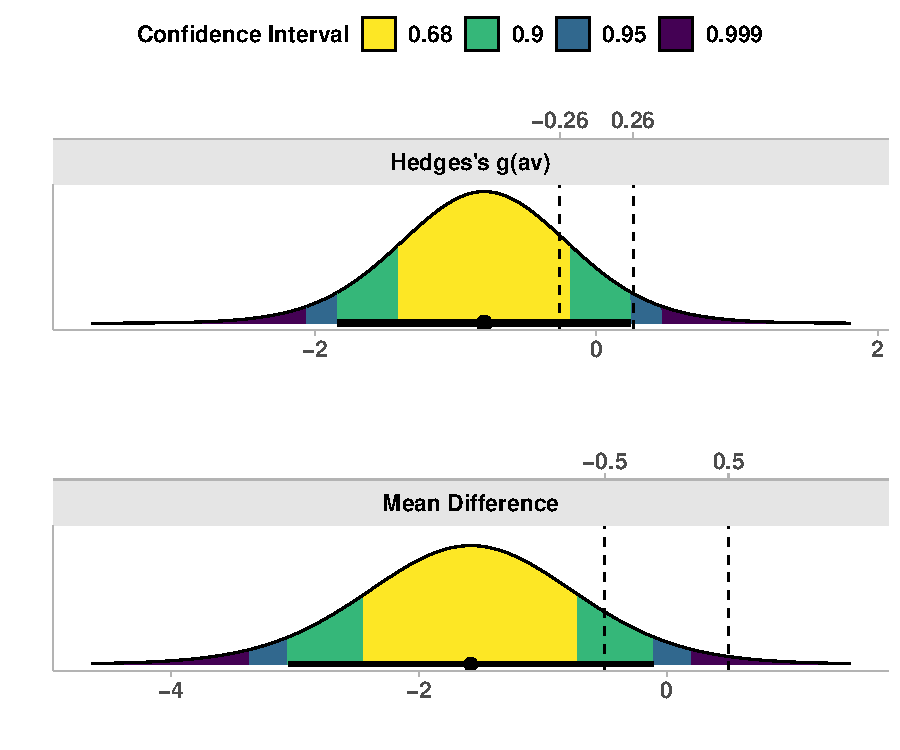
\includegraphics{avocado-quarto_files/figure-pdf/cdplot-1.pdf}

}

\caption{Example of consonance density plot.}

\end{figure}

\newpage

The shading pattern can be modified with the \texttt{ci\_shades}.

\begin{Shaded}
\begin{Highlighting}[]
\FunctionTok{plot}\NormalTok{(res1, }\AttributeTok{type =} \StringTok{"cd"}\NormalTok{,}
     \AttributeTok{ci\_shades =} \FunctionTok{c}\NormalTok{(.}\DecValTok{9}\NormalTok{,.}\DecValTok{95}\NormalTok{))}
\end{Highlighting}
\end{Shaded}

\begin{figure}[H]

{\centering 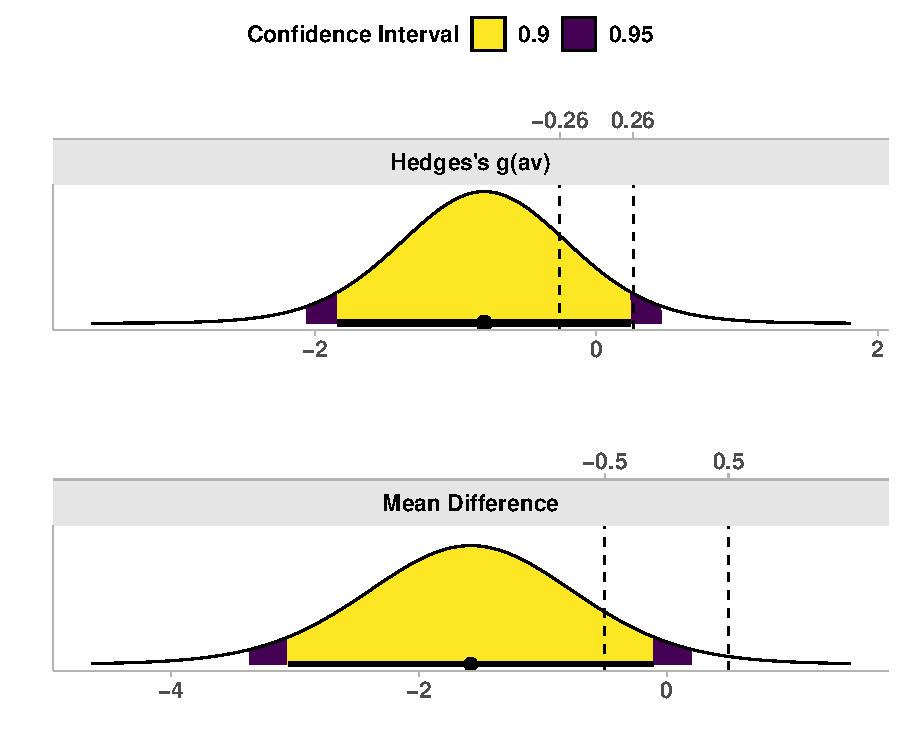
\includegraphics{avocado-quarto_files/figure-pdf/shadeplot-1.pdf}

}

\caption{Demonstrating the shading in plot method.}

\end{figure}

\newpage

Consonance plots, where all confidence intervals can be simultaneous
plotted, can also be produced. The advantage here is multiple confidence
interval lines can plotted at once.

\begin{Shaded}
\begin{Highlighting}[]
\FunctionTok{plot}\NormalTok{(res1, }\AttributeTok{type =} \StringTok{"c"}\NormalTok{,}
     \AttributeTok{ci\_lines =}  \FunctionTok{c}\NormalTok{(.}\DecValTok{9}\NormalTok{,.}\DecValTok{95}\NormalTok{))}
\end{Highlighting}
\end{Shaded}

\begin{figure}[H]

{\centering 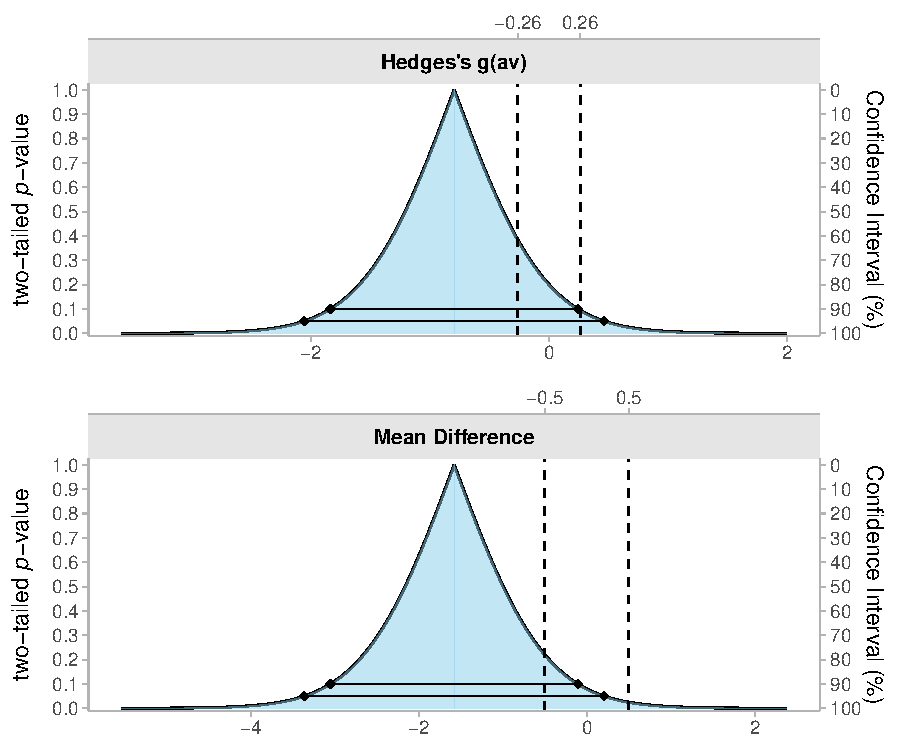
\includegraphics{avocado-quarto_files/figure-pdf/conplot-1.pdf}

}

\caption{Example of consonance plot.}

\end{figure}

\newpage

\hypertarget{paired-sample}{%
\subsection{Paired Sample}\label{paired-sample}}

To perform TOST on paired samples, the process does not change much. We
could process the test the same way by providing a formula. All we would
need to then is change \texttt{paired} to TRUE.

\begin{Shaded}
\begin{Highlighting}[]
\NormalTok{res2 }\OtherTok{=} \FunctionTok{t\_TOST}\NormalTok{(}
  \AttributeTok{formula =}\NormalTok{ extra }\SpecialCharTok{\textasciitilde{}}\NormalTok{ group,}
  \AttributeTok{data =}\NormalTok{ sleep,}
  \AttributeTok{paired =} \ConstantTok{TRUE}\NormalTok{,}
  \AttributeTok{eqb =}\NormalTok{ .}\DecValTok{5}
\NormalTok{)}
\NormalTok{res2}
\end{Highlighting}
\end{Shaded}

\begin{verbatim}

Paired t-test

The equivalence test was non-significant, t(9) = -2.8, p = 0.99
The null hypothesis test was significant, t(9) = -4.06p < 0.01
NHST: reject null significance hypothesis that the effect is equal to zero 
TOST: don't reject null equivalence hypothesis

TOST Results 
                t df p.value
t-test     -4.062  9   0.003
TOST Lower -2.777  9   0.989
TOST Upper -5.348  9 < 0.001

Effect Sizes 
              Estimate    SE               C.I. Conf. Level
Raw             -1.580 0.389   [-2.293, -0.867]         0.9
Hedges's g(z)   -1.174 0.411 [-1.8046, -0.4977]         0.9
Note: SMD confidence intervals are an approximation. See vignette("SMD_calcs").
\end{verbatim}

\begin{Shaded}
\begin{Highlighting}[]
\NormalTok{res2\_simple }\OtherTok{=} \FunctionTok{simple\_htest}\NormalTok{(}
  \AttributeTok{formula =}\NormalTok{ extra }\SpecialCharTok{\textasciitilde{}}\NormalTok{ group,}
  \AttributeTok{data =}\NormalTok{ sleep,}
  \AttributeTok{paired =} \ConstantTok{TRUE}\NormalTok{,}
  \AttributeTok{alternative =} \StringTok{"equivalence"}\NormalTok{,}
  \CommentTok{\# set hypothesis test}
  \AttributeTok{mu =}\NormalTok{ .}\DecValTok{5}
\NormalTok{)}
\NormalTok{res2\_simple}
\end{Highlighting}
\end{Shaded}

\begin{verbatim}

    Paired t-test

data:  extra by group
t = -2.7766, df = 9, p-value = 0.9892
alternative hypothesis: equivalence
null values:
mean difference mean difference 
           -0.5             0.5 
90 percent confidence interval:
 -2.2930053 -0.8669947
sample estimates:
mean difference 
          -1.58 
\end{verbatim}

\newpage

However, we may have two vectors of data that are paired. So instead we
may want to just provide those separately rather than using a data set
and setting the formula. This can be demonstrated with the ``bugs''
data.

\begin{Shaded}
\begin{Highlighting}[]
\NormalTok{res3 }\OtherTok{=} \FunctionTok{t\_TOST}\NormalTok{(}\AttributeTok{x =}\NormalTok{ bugs}\SpecialCharTok{$}\NormalTok{LDHF,}
              \AttributeTok{y =}\NormalTok{ bugs}\SpecialCharTok{$}\NormalTok{LDLF,}
              \AttributeTok{paired =} \ConstantTok{TRUE}\NormalTok{,}
              \AttributeTok{eqb =} \DecValTok{1}\NormalTok{)}
\NormalTok{res3}
\end{Highlighting}
\end{Shaded}

\begin{verbatim}

Paired t-test

The equivalence test was non-significant, t(90) = 2.66, p = 1
The null hypothesis test was significant, t(90) = 6.649p < 0.01
NHST: reject null significance hypothesis that the effect is equal to zero 
TOST: don't reject null equivalence hypothesis

TOST Results 
                t df p.value
t-test      6.649 90 < 0.001
TOST Lower 10.642 90 < 0.001
TOST Upper  2.655 90   0.995

Effect Sizes 
              Estimate     SE             C.I. Conf. Level
Raw             1.6648 0.2504  [1.2487, 2.081]         0.9
Hedges's g(z)   0.6911 0.1167 [0.4987, 0.8802]         0.9
Note: SMD confidence intervals are an approximation. See vignette("SMD_calcs").
\end{verbatim}

\newpage

Additionally, a MET, instead of equivalence testing, can be performed
with the \texttt{hypothesis} argument set to ``MET''. With this setting,
the hypothesis being tested is whether the effect is \emph{greater} than
the equivalence bound.

\begin{Shaded}
\begin{Highlighting}[]
\NormalTok{res3a }\OtherTok{=} \FunctionTok{t\_TOST}\NormalTok{(}\AttributeTok{x =}\NormalTok{ bugs}\SpecialCharTok{$}\NormalTok{LDHF,}
               \AttributeTok{y =}\NormalTok{ bugs}\SpecialCharTok{$}\NormalTok{LDLF,}
               \AttributeTok{paired =} \ConstantTok{TRUE}\NormalTok{,}
               \AttributeTok{hypothesis =} \StringTok{"MET"}\NormalTok{,}
               \AttributeTok{eqb =} \DecValTok{1}\NormalTok{)}
\NormalTok{res3a}
\end{Highlighting}
\end{Shaded}

\begin{verbatim}

Paired t-test

The minimal effect test was significant, t(90) = 10.64, p < 0.01
The null hypothesis test was significant, t(90) = 6.649p < 0.01
NHST: reject null significance hypothesis that the effect is equal to zero 
TOST: reject null MET hypothesis

TOST Results 
                t df p.value
t-test      6.649 90 < 0.001
TOST Lower 10.642 90       1
TOST Upper  2.655 90   0.005

Effect Sizes 
              Estimate     SE             C.I. Conf. Level
Raw             1.6648 0.2504  [1.2487, 2.081]         0.9
Hedges's g(z)   0.6911 0.1167 [0.4987, 0.8802]         0.9
Note: SMD confidence intervals are an approximation. See vignette("SMD_calcs").
\end{verbatim}

\begin{Shaded}
\begin{Highlighting}[]
\NormalTok{res3a\_simple }\OtherTok{=} \FunctionTok{simple\_htest}\NormalTok{(}\AttributeTok{x =}\NormalTok{ bugs}\SpecialCharTok{$}\NormalTok{LDHF,}
               \AttributeTok{y =}\NormalTok{ bugs}\SpecialCharTok{$}\NormalTok{LDLF,}
               \AttributeTok{paired =} \ConstantTok{TRUE}\NormalTok{,}
               \AttributeTok{alternative =} \StringTok{"m"}\NormalTok{,}
               \AttributeTok{mu =} \DecValTok{1}\NormalTok{)}
\NormalTok{res3a\_simple}
\end{Highlighting}
\end{Shaded}

\begin{verbatim}

    Paired t-test

data:  x and y
t = 2.6551, df = 90, p-value = 0.004689
alternative hypothesis: minimal.effect
null values:
mean difference mean difference 
             -1               1 
90 percent confidence interval:
 1.248675 2.080996
sample estimates:
mean difference 
       1.664835 
\end{verbatim}

The data would indicate that we should accept the MET hypothesis.

\newpage

\hypertarget{one-sample-t-test}{%
\subsection{One Sample t-test}\label{one-sample-t-test}}

In other cases we may have a one sample test. If that is the case, only
\texttt{x} argument for the data is needed. This is useful in situations
where you may have hypotheses to test about a single samples mean. In
order for the two-sample test to be correct, we also need to supply the
\texttt{mu} argument. In the example below, we hypothesize that the mean
of \texttt{LDHF} is not more than 1.5 points greater or less than 7.
With the way the \texttt{mu} and \texttt{eqb} arguments are set, we are
testing whether the mean of \texttt{LDHF} is significantly different
from 7.5 (two-tailed tests) and (\(\pm\)) than 1.5 points 7.5 as well
(equivalence bounds at 5.5 and 8.5).

\begin{Shaded}
\begin{Highlighting}[]
\NormalTok{res4 }\OtherTok{=} \FunctionTok{t\_TOST}\NormalTok{(}\AttributeTok{x =}\NormalTok{ bugs}\SpecialCharTok{$}\NormalTok{LDHF,}
              \AttributeTok{hypothesis =} \StringTok{"EQU"}\NormalTok{,}
              \AttributeTok{mu =} \FloatTok{7.5}\NormalTok{,}
              \AttributeTok{eqb =} \FunctionTok{c}\NormalTok{(}\FloatTok{5.5}\NormalTok{,}\FloatTok{8.5}\NormalTok{))}
\NormalTok{res4}
\end{Highlighting}
\end{Shaded}

\begin{verbatim}

One Sample t-test

The equivalence test was significant, t(90) = -4.2, p < 0.01
The null hypothesis test was non-significant, t(90) = -0.458p = 0.65
NHST: don't reject null significance hypothesis that the effect is equal to 7.5 
TOST: reject null equivalence hypothesis

TOST Results 
                 t df p.value
t-test     -0.4577 90   0.648
TOST Lower  7.1156 90 < 0.001
TOST Upper -4.2444 90 < 0.001

Effect Sizes 
           Estimate     SE              C.I. Conf. Level
Raw        -0.12088 0.2641   [6.9402, 7.818]         0.9
Hedges's g -0.04758 0.1049 [-0.2185, 0.1236]         0.9
Note: SMD confidence intervals are an approximation. See vignette("SMD_calcs").
\end{verbatim}

We would conclude that \texttt{LDHF} is practically equivalent to the
hypothesized mean (7.5).

\newpage

\hypertarget{using-summary-statistics}{%
\subsection{Using Summary Statistics}\label{using-summary-statistics}}

In some cases you may only have access to the summary statistics (e.g.,
when reviewing an article or attempting to perform a meta-analysis).
Therefore, I created a function, \texttt{tsum\_TOST}, to perform the
same tests just based on the summary statistics. This involves providing
the function with a number of different arguments.

\begin{itemize}
\tightlist
\item
  \texttt{n1\ \&\ n2} the sample sizes (only n1 needs to be provided for
  one sample case)
\item
  \texttt{m1\ \&\ m2} the sample means
\item
  \texttt{sd1\ \&\ sd2} the sample standard deviation
\item
  \texttt{r12} the correlation between each if paired is set to
  TRUE\footnote{The \texttt{extract\_r\_paired} function can be used if
    the correlation between paired observations is not readily
    available.}
\end{itemize}

The results from the \texttt{bugs} example can be replicated with the
\texttt{tsum\_TOST}:

\begin{Shaded}
\begin{Highlighting}[]
\NormalTok{res\_tsum }\OtherTok{=} \FunctionTok{tsum\_TOST}\NormalTok{(}
  \AttributeTok{m1 =} \FunctionTok{mean}\NormalTok{(bugs}\SpecialCharTok{$}\NormalTok{LDHF, }\AttributeTok{na.rm=}\ConstantTok{TRUE}\NormalTok{), }\AttributeTok{sd1 =} \FunctionTok{sd}\NormalTok{(bugs}\SpecialCharTok{$}\NormalTok{LDHF, }\AttributeTok{na.rm=}\ConstantTok{TRUE}\NormalTok{),}
  \AttributeTok{n1 =} \FunctionTok{length}\NormalTok{(}\FunctionTok{na.omit}\NormalTok{(bugs}\SpecialCharTok{$}\NormalTok{LDHF)),}
  \AttributeTok{hypothesis =} \StringTok{"EQU"}\NormalTok{, }\AttributeTok{smd\_ci =} \StringTok{"t"}\NormalTok{, }\AttributeTok{eqb =} \FunctionTok{c}\NormalTok{(}\FloatTok{5.5}\NormalTok{, }\FloatTok{8.5}\NormalTok{)}
\NormalTok{)}

\NormalTok{res\_tsum}
\end{Highlighting}
\end{Shaded}

\begin{verbatim}

One-sample t-Test

The equivalence test was significant, t(90) = -4.244, p = 2.66e-05
The null hypothesis test was significant, t(90) = 27.942, p = 3.91e-46
NHST: reject null significance hypothesis that the effect is equal to zero 
TOST: reject null equivalence hypothesis

TOST Results 
                t df p.value
t-test     27.942 90 < 0.001
TOST Lower  7.116 90 < 0.001
TOST Upper -4.244 90 < 0.001

Effect Sizes 
           Estimate     SE             C.I. Conf. Level
Raw           7.379 0.2641  [6.9402, 7.818]         0.9
Hedges's g    2.905 0.2395 [2.4289, 3.3804]         0.9
Note: SMD confidence intervals are an approximation. See vignette("SMD_calcs").
\end{verbatim}

\newpage

\hypertarget{robust-methods-for-equivalence-testing}{%
\section{Robust Methods for Equivalence
Testing}\label{robust-methods-for-equivalence-testing}}

In some cases, the use of t-test may be less than ideal. Any serious
violation to the assumptions of a t-test (e.g., normality or
homoscedasticity) could greatly inflate the type 1 error rate of TOST.
Therefore, it may be useful to explore alternatives to the t-test for
TOST that either do not have those assumptions or are robust to
violating those assumptions.

The TOSTER package currently provides 5 robust alternatives to the
t-test for TOST. First, there is the \texttt{wilcox\_TOST} function
which uses the Wilcoxon-Mann-Whitney (WMW) type tests (i.e.,
\texttt{wilcox.test}) to perform TOST as a test of symmetry. Second,
there is the \texttt{boot\_t\_TOST} function which uses the bootstrap
method outlined by Efron and Tibshirani
(\protect\hyperlink{ref-efron93}{1993}). Third, there is the
\texttt{log\_TOST} function which performs log-transformed t-tests,
which is a parametric approach commonly used in pharmaceutical
bioequivalence studies on ratio data (\protect\hyperlink{ref-he2022}{He
et al. 2022}). Fourth, there is the \texttt{boot\_log\_TOST} function
which uses the same bootstrap method outlined by Efron and Tibshirani
(\protect\hyperlink{ref-efron93}{1993}) but on the log-transformed data,
which is more robust than parametric log t-test
(\protect\hyperlink{ref-he2022}{He et al. 2022}). Fifth, the
Brunner-Munzel tests which is another non-parametric test that can be
thought of as an alternative to the WMW tests
(\protect\hyperlink{ref-karch2021}{Karch 2021}).

In the following sections, I will briefly outline the available robust
TOST functions within the TOSTER package.

\hypertarget{tests-of-symmetry-rank-based-tests}{%
\subsection{Tests of Symmetry (rank based
tests)}\label{tests-of-symmetry-rank-based-tests}}

The WMW group of tests (e.g., Mann-Whitney U-test) provide a
non-parametric test of differences between groups, or within samples,
based on \emph{ranks}. This provides a test of location shift, which is
a fancy way of saying differences in the center of the distribution
(e.g., in parametric tests the location is the mean). Within the TOST
framework, there are two separate tests of directional location shift to
determine if the location shift is within (equivalence) or outside
(minimal effect) the equivalence bounds. Many researchers mistakenly
think these are tests of medians, but this is not the case (See Divine
et al. (\protect\hyperlink{ref-median_test}{2018}) for details). Using a
WMW-based TOST is useful for testing whether the differences between
groups/conditions is symmetric around the equivalence bounds\footnote{Care
  should be taken when considering paired samples; a test on the rank
  transformed data (\protect\hyperlink{ref-kornbrot1990rank}{Kornbrot
  1990}) or another robust test may be more prudent.}. For equivalence
testing, the TOST would be testing whether there is asymmetry towards no
effect with a null hypothesis of symmetry at the equivalence bound.

In the TOSTER package, we accomplish this ``test of symmetry'' with the
\texttt{wilcox\_TOST} function. This function operates in an extremely
similar implementation to the \texttt{t\_TOST} function. The exact
calculations utilized in this function can be explored via the
documentation of the \texttt{wilcox.test} function. A standardized mean
difference (SMD) is \emph{not} calculated in this function since this
would be an inappropriate measure of effect size alongside the
non-parametric test statistics. Instead, a standardized effect size
(SES) is calculated for \emph{all} types of comparisons (e.g., two
sample, one sample, and paired samples). The function can produce a
rank-biserial correlation (\protect\hyperlink{ref-Kerby_2014}{Kerby
2014}), a WMW Odds (\protect\hyperlink{ref-wmwodds}{O'Brien and
Castelloe 2006}), or a ``common language effect size''
(\protect\hyperlink{ref-Kerby_2014}{Kerby 2014}) (Also known as the
non-parametric probability of superiority, or concordance
probability).\footnote{There is no plotting capability at this time for
  the output of this function.}

\newpage

As an example, we can use the sleep data to make a non-parametric
comparison of equivalence.

\begin{Shaded}
\begin{Highlighting}[]
\NormalTok{test1 }\OtherTok{=} \FunctionTok{wilcox\_TOST}\NormalTok{(}\AttributeTok{formula =}\NormalTok{ extra }\SpecialCharTok{\textasciitilde{}}\NormalTok{ group,}
                      \AttributeTok{data =}\NormalTok{ sleep,}
                      \AttributeTok{paired =} \ConstantTok{FALSE}\NormalTok{,}
                      \AttributeTok{eqb =}\NormalTok{ .}\DecValTok{5}\NormalTok{)}
\FunctionTok{print}\NormalTok{(test1)}
\end{Highlighting}
\end{Shaded}

\begin{verbatim}

Wilcoxon rank sum test with continuity correction

The equivalence test was non-significant W = 20.000, p = 8.94e-01
The null hypothesis test was non-significant W = 25.500, p = 6.93e-02
NHST: don't reject null significance hypothesis that the effect is equal to zero 
TOST: don't reject null equivalence hypothesis

TOST Results 
           Test Statistic p.value
NHST                 25.5   0.069
TOST Lower           34.0   0.894
TOST Upper           20.0   0.013

Effect Sizes 
                          Estimate               C.I. Conf. Level
Median of Differences       -1.346       [-3.4, -0.1]         0.9
Rank-Biserial Correlation   -0.490 [-0.7493, -0.1005]         0.9
\end{verbatim}

Based on these results, we would have conclude there is no significant
difference but not equivalent differences either (i.e., inconclusive
result).

\newpage

\hypertarget{bootstrap-tost}{%
\subsection{Bootstrap TOST}\label{bootstrap-tost}}

The bootstrap refers to resampling with replacement and can be used for
statistical estimation and inference. Bootstrapping techniques are very
useful because they are considered somewhat robust to the violations of
assumptions for a simple t-test and provide better estimations of SMDs
(\protect\hyperlink{ref-Kirby2013}{Kirby and Gerlanc 2013}). Therefore,
I added a bootstrapping function, \texttt{boot\_t\_TOST}, to the package
to provide another robust alternative to the \texttt{t\_TOST} function.

In this function we provide a percentile bootstrap solution outlined by
Efron and Tibshirani (\protect\hyperlink{ref-efron93}{1993}) (see
chapter 16, page 220). The bootstrapped p-values are derived from the
``studentized'' version of a test of mean differences
(\protect\hyperlink{ref-efron93}{Efron and Tibshirani 1993}). Overall,
the results should be similar to the results of \texttt{t\_TOST}.
\textbf{However}, for paired samples, the Cohen's d(rm) effect size
\emph{cannot} be calculated by this function.

\hypertarget{two-sample-algorithm}{%
\subsubsection{Two Sample Algorithm}\label{two-sample-algorithm}}

The steps by which the bootstrapping occurs are fairly simple.

\begin{enumerate}
\def\labelenumi{\arabic{enumi}.}
\item
  Form B bootstrap data sets from x* and y* wherein x* is sampled with
  replacement from \(\tilde x_1,\tilde x_2, ... \tilde x_n\) and y* is
  sampled with replacement from
  \(\tilde y_1,\tilde y_2, ... \tilde y_n\)
\item
  t is then evaluated on each sample, but the mean of each sample (y or
  x) and the overall average (z) are subtracted from each (i.e., null
  distribution is formed)
\end{enumerate}

\[
t(z^{*b}) = \frac {(\bar x^*-\bar x - \bar z) - (\bar y^*-\bar y - \bar z)}{\sqrt {sd_y^*/n_y + sd_x^*/n_x}}
\]

\begin{enumerate}
\def\labelenumi{\arabic{enumi}.}
\setcounter{enumi}{2}
\tightlist
\item
  An approximate p-value can then be calculated as the number of
  bootstrapped results greater than the observed t-statistic from the
  sample.
\end{enumerate}

\[
p_{boot} = \frac {\#t(z^{*b}) \ge t_{sample}}{B}
\]

The same process is completed for the one sample case but with the one
sample solution for the equation outlined by \(t(z^{*b})\). The paired
sample case in this bootstrap procedure is equivalent to the one sample
solution because the test is based on the difference scores.

\newpage

\hypertarget{example-of-bootsrapping}{%
\subsubsection{Example of Bootsrapping}\label{example-of-bootsrapping}}

We can use the sleep data to see an example of the bootstrapped results.
If you plot the bootstrap samples, it will show how the resampling via
bootstrapping indicates the instability of Hedges' d(z). Just looking at
the printed results you will notice some differences between confidence
intervals from the bootstrapped result and the t-test.

\begin{Shaded}
\begin{Highlighting}[]
\FunctionTok{set.seed}\NormalTok{(}\DecValTok{891111}\NormalTok{)}
\NormalTok{test1 }\OtherTok{=} \FunctionTok{boot\_t\_TOST}\NormalTok{(}\AttributeTok{formula =}\NormalTok{ extra }\SpecialCharTok{\textasciitilde{}}\NormalTok{ group,}
                    \AttributeTok{data =}\NormalTok{ sleep,}
                    \AttributeTok{paired =} \ConstantTok{TRUE}\NormalTok{,}
                    \AttributeTok{eqb =}\NormalTok{ .}\DecValTok{5}\NormalTok{,}
                    \AttributeTok{R =} \DecValTok{999}\NormalTok{)}


\FunctionTok{print}\NormalTok{(test1)}
\end{Highlighting}
\end{Shaded}

\begin{verbatim}

Bootstrapped Paired t-test

The equivalence test was non-significant, t(9) = -2.777, p = 1e+00
The null hypothesis test was significant, t(9) = -4.062, p = 0e+00
NHST: reject null significance hypothesis that the effect is equal to zero 
TOST: don't reject null equivalence hypothesis

TOST Results 
                t df p.value
t-test     -4.062  9 < 0.001
TOST Lower -2.777  9       1
TOST Upper -5.348  9 < 0.001

Effect Sizes 
              Estimate     SE               C.I. Conf. Level
Raw             -1.580 0.3699    [-2.26, -1.038]         0.9
Hedges's g(z)   -1.174 0.6491 [-2.7507, -0.9285]         0.9
Note: percentile bootstrap method utilized.
\end{verbatim}

\newpage

\hypertarget{log-tost}{%
\subsection{Log TOST}\label{log-tost}}

The natural logarithmic (log) transformation is often utilized to
stabilize the variance of a measure, and it often provides the best
approximation of the normal distribution
(\protect\hyperlink{ref-logtest}{Bland and Altman 1996}). However,
another, less often reported, advantage of the log transformation is
that the back transformation of the differences of the log-transformed
data is a \emph{ratio} (\protect\hyperlink{ref-logtest}{Bland and Altman
1996}). For example, if we had a two samples (x \& y) with an geometric
mean\footnote{The mean of log-transformed data is the \emph{geometric}
  not \emph{arithmetic} mean. I highly recommend reading Bland and
  Altman (\protect\hyperlink{ref-logtest}{1996}) and Caldwell and
  Cheuvront (\protect\hyperlink{ref-caldwell2019basic}{2019}) for more
  details} or 7 and 10.5, x and y respectively in the code below, we
could represent the differences as ratio of y:x where y is 1.5 times
greater than x.

\begin{Shaded}
\begin{Highlighting}[]
\NormalTok{x }\OtherTok{=} \DecValTok{7}\NormalTok{; y }\OtherTok{=} \FloatTok{10.5}
\FunctionTok{log}\NormalTok{(y) }\SpecialCharTok{{-}} \FunctionTok{log}\NormalTok{(x)}
\end{Highlighting}
\end{Shaded}

\begin{verbatim}
[1] 0.4054651
\end{verbatim}

\begin{Shaded}
\begin{Highlighting}[]
\FunctionTok{log}\NormalTok{(y}\SpecialCharTok{/}\NormalTok{x)}
\end{Highlighting}
\end{Shaded}

\begin{verbatim}
[1] 0.4054651
\end{verbatim}

\begin{Shaded}
\begin{Highlighting}[]
\FunctionTok{exp}\NormalTok{(}\FunctionTok{log}\NormalTok{(y) }\SpecialCharTok{{-}} \FunctionTok{log}\NormalTok{(x))}
\end{Highlighting}
\end{Shaded}

\begin{verbatim}
[1] 1.5
\end{verbatim}

\begin{Shaded}
\begin{Highlighting}[]
\NormalTok{y}\SpecialCharTok{/}\NormalTok{x}
\end{Highlighting}
\end{Shaded}

\begin{verbatim}
[1] 1.5
\end{verbatim}

The log transformation thereby acts as a useful tool help tame data into
conforming to the normality assumption, and makes the interpretation
fairly simple. In addition, some regulatory agencies, such as the United
States Food and Drug Administration (FDA)
(\protect\hyperlink{ref-fda}{Food and Drug Administration 2014}),
specifically require bioequivalence studies to report the geometric
means and make statistical comparisons on the log transformed data
(\protect\hyperlink{ref-he2022}{He et al. 2022}). In pharmaceutical
reserach, bioequivalence testing involves determining whether two drugs,
a test drug and a reference drug, have the same rate and extent of
absorption in the body. This is typically accomplished by testing
whether the blood concentrations of the drug after administration of the
test drug are sufficiently close to the blood concentrations after
administration of the reference drug. If the two drugs are
bioequivalent, they can be used interchangeably. The area under the
curve (AUC) is the measure of the extent of absorption, and the peak
concentration is the measure of the rate of absorption. In order to
determine bioequivalence, the AUC and peak concentration of the test
drug must be within a certain percentage of the AUC and peak
concentration of the reference drug.

In my personal experience as a physiologist, it is not uncommon that
biological/physiological phenomenon present have longer right-tailed
distributions, and are often adequately normalized with a natural log
transformation. The additional advantage is the how equivalence bounds
can, almost, be universally applied when making comparisons on the log
scale. The FDA considers to drugs to be bioequivalent when the maximal
concentration and AUC differences between drugs are less than 1.25. To
put it another way, ratio between two means must be between 1.25 and 0.8
(i.e., 1/1.25) (\protect\hyperlink{ref-fda}{Food and Drug Administration
2014}).

Therefore, I have implemented two functions to allow for the comparison
of data that is believed to be left skewed (long right tail), and is on
a ratio scale\footnote{Ratio scale means the outcome is measured on a
  numerical scale that has equal distances between adjacent values and
  true zero.}. The first function is a parametric t-test on the log
transformed scale while the second function is a bootstrapping test
which is more robust than parametric version
(\protect\hyperlink{ref-he2022}{He et al. 2022}).

\hypertarget{example-of-log-tost}{%
\subsubsection{Example of Log TOST}\label{example-of-log-tost}}

The \texttt{log\_TOST} function is almost exactly the same as the
\texttt{t\_TOST} function. First, the primary differences is that it
only accepts paired and two sample comparisons. One sample tests are not
support (i.e., there is no ratio to calculate). Second, standardized
mean differences are not calculated, but a ratio of means is instead
reported {[}Lajeunesse
(\protect\hyperlink{ref-lajeunesse2015bias}{2015}){]}\footnote{Also,
  referred to as a ``response ratio'' in ecology. Like an SMD, the
  response ratio can be utilized in meta-analysis.}. Third, the default
equivalence bounds are by default set to the FDA standards (i.e.,
\texttt{eqb\ =\ 1.25}), but can be changed by the user\footnote{Only one
  value needs to be supplied to eqb; the reciprocal value of eqb is
  taken as the other equivalence bound. For example, if
  \texttt{eqb\ \ =\ 0.85} then the upper equivalence bound is 1/0.85
  (\textasciitilde1.333)} .

As an example we can use the \texttt{mtcars} data to compare the type of
transmission (\texttt{am}) effects on the gas mileage (\texttt{mpg}). We
can see from the data below there are significant, non-equivalent,
differences in mpg between transmission types.

\begin{Shaded}
\begin{Highlighting}[]
\FunctionTok{log\_TOST}\NormalTok{(mpg }\SpecialCharTok{\textasciitilde{}}\NormalTok{ am, }\AttributeTok{data =}\NormalTok{ mtcars)}
\end{Highlighting}
\end{Shaded}

\begin{verbatim}

Log-transformed Welch Two Sample t-test

The equivalence test was non-significant, t(23.96) = -1.363, p = 9.07e-01
The null hypothesis test was significant, t(23.96) = -3.826, p = 8.19e-04
NHST: reject null significance hypothesis that the effect is equal to one 
TOST: don't reject null equivalence hypothesis

TOST Results 
                t    df p.value
t-test     -3.826 23.96 < 0.001
TOST Lower -1.363 23.96   0.907
TOST Upper -6.288 23.96 < 0.001

Effect Sizes 
                 Estimate      SE               C.I. Conf. Level
log(Means Ratio)  -0.3466 0.09061 [-0.5017, -0.1916]         0.9
Means Ratio        0.7071      NA   [0.6055, 0.8256]         0.9
\end{verbatim}

\newpage

\hypertarget{example-of-bootstrap-log-tost}{%
\subsubsection{Example of Bootstrap Log
TOST}\label{example-of-bootstrap-log-tost}}

The bootstrap version of \texttt{log\_TOST}, \texttt{boot\_log\_TOST},
uses the same bootstrapping method detailed above
(\texttt{boot\_t\_TOST}), but it uses the log-transformed values and
produces the ratio of means as the effect size.

\begin{Shaded}
\begin{Highlighting}[]
\FunctionTok{boot\_log\_TOST}\NormalTok{(mpg }\SpecialCharTok{\textasciitilde{}}\NormalTok{ am, }\AttributeTok{data =}\NormalTok{ mtcars, }\AttributeTok{R=}\DecValTok{999}\NormalTok{)}
\end{Highlighting}
\end{Shaded}

\begin{verbatim}

Bootstrapped Log Welch Two Sample t-test

The equivalence test was non-significant, t(23.96) = -1.363, p = 9.57e-01
The null hypothesis test was significant, t(23.96) = -3.826, p = 0e+00
NHST: reject null significance hypothesis that the effect is equal to 1 
TOST: don't reject null equivalence hypothesis

TOST Results 
                t    df p.value
t-test     -3.826 23.96 < 0.001
TOST Lower -1.363 23.96   0.957
TOST Upper -6.288 23.96 < 0.001

Effect Sizes 
                 Estimate      SE               C.I. Conf. Level
log(Means Ratio)  -0.3466 0.08634 [-0.4871, -0.2039]         0.9
Means Ratio        0.7071 0.06119   [0.6144, 0.8156]         0.9
Note: percentile bootstrap method utilized.
\end{verbatim}

From this analysis, we would conclude there is a significant effect that
is not practically equivalent.

\newpage

\hypertarget{equivalence-testing-with-anovas}{%
\section{Equivalence Testing with
ANOVAs}\label{equivalence-testing-with-anovas}}

Many researchers utilize ANOVA as an omnibus test for the
absence/presence of effects before inspecting multiple pairwise
comparisons. This is very useful when implementing factorial designs
wherein multiple experimental factors are tested and/or manipulated. As
Campbell and Lakens (\protect\hyperlink{ref-Campbell_2021}{2021})
suggest, the lack of a significant result at the ANOVA-level does not
necessarily indicate that a factor or interaction of factors have no
effect. However, Campbell and Lakens
(\protect\hyperlink{ref-Campbell_2021}{2021}) only suggest an
equivalence test for one-way ANOVAs and therefore exclude multi-factor
or factorial ANOVAs. Therefore, I have extended the work of Campbell and
Lakens (\protect\hyperlink{ref-Campbell_2021}{2021}) to include
functions that allow for equivalence testing of the partial \(\eta^2\)
(eta-squared) effect size from ANOVAs.

\hypertarget{f-test-calculations}{%
\subsection{F-test Calculations}\label{f-test-calculations}}

Statistical equivalence testing\footnote{Also called ``omnibus
  non-inferiority testing'' by Campbell and Lakens
  (\protect\hyperlink{ref-Campbell_2021}{2021})} for \emph{F}-tests are
special use case of the cumulative distribution function of the
non-central \emph{F} distribution. As Campbell and Lakens
(\protect\hyperlink{ref-Campbell_2021}{2021}) states, this type of
statistical test answers the question: ``Can we reject the hypothesis
that the total proportion of variance in outcome Y attributable to X is
greater than or equal to the equivalence bound \(\Delta\)?''

\hypertarget{hypothesis-tests}{%
\subsubsection{Hypothesis Tests}\label{hypothesis-tests}}

\[
H_0 =  1 > \eta^2_p \geq \Delta
\]

\[
H_1 =  0 \geq \eta^2_p < \Delta
\]

In TOSTER, I have gone a tad farther than Campbell and Lakens
(\protect\hyperlink{ref-Campbell_2021}{2021}), and have included a
calculation for a generalization of the non-centrality parameter that
allows the equivalence test for \emph{F}-tests to be applied to variety
of designs.

Campbell and Lakens (\protect\hyperlink{ref-Campbell_2021}{2021})
calculate the \emph{p}-value as:

\[
p = p_f(F; J-1, N-J, \frac{N \cdot \Delta}{1-\Delta})
\]

The non-centrality parameter (ncp = \(\lambda\)) can be calculated with
the equivalence bound and the degrees of freedom:

\[
\lambda_{eq} = \frac{\Delta}{1-\Delta} \cdot(df_1 + df_2 +1)
\]

\newpage

The \emph{p}-value for the equivalence test (\(p_{eq}\)) could then be
calculated from traditional ANOVA results and the distribution function:

\[
p_{eq} = p_f(F; df_1, df_2, \lambda_{eq})
\]

\hypertarget{example-of-equivalence-anova-testing}{%
\subsection{Example of Equivalence ANOVA
Testing}\label{example-of-equivalence-anova-testing}}

Using the \texttt{InsectSprays} data set in R and the base R
\texttt{aov} function, I can demonstrate how this omnibus equivalence
testing can be applied with TOSTER. From the initial analysis we an see
a clear ``significant'' effect (very small p-value) of the inspect
spray. However, we \emph{may} be interested in testing if the effect is
practically equivalent. I will arbitrarily set the equivalence bound to
a partial eta-squared of 0.35 (\(H_0: \eta^2_p > 0.35\)).

\begin{Shaded}
\begin{Highlighting}[]
\FunctionTok{data}\NormalTok{(}\StringTok{"InsectSprays"}\NormalTok{)}
\NormalTok{aovtest }\OtherTok{=} \FunctionTok{aov}\NormalTok{(count }\SpecialCharTok{\textasciitilde{}}\NormalTok{ spray, }\AttributeTok{data =}\NormalTok{ InsectSprays)}
\FunctionTok{anova}\NormalTok{(aovtest)}
\end{Highlighting}
\end{Shaded}

\begin{verbatim}
Analysis of Variance Table

Response: count
          Df Sum Sq Mean Sq F value    Pr(>F)    
spray      5 2668.8  533.77  34.702 < 2.2e-16 ***
Residuals 66 1015.2   15.38                      
---
Signif. codes:  0 '***' 0.001 '**' 0.01 '*' 0.05 '.' 0.1 ' ' 1
\end{verbatim}

We can then use the information in the table above to perform an
equivalence test using the \texttt{equ\_ftest} function. This function
returns an object of the S3 class \texttt{htest} and the output will
look very familiar to that of the t-test. The main difference is the
estimates, and confidence interval, are for partial \(\eta^2_p\).

\begin{Shaded}
\begin{Highlighting}[]
\FunctionTok{equ\_ftest}\NormalTok{(}\AttributeTok{Fstat =} \FloatTok{34.70228}\NormalTok{,  }\AttributeTok{df1 =} \DecValTok{5}\NormalTok{, }\AttributeTok{df2 =} \DecValTok{66}\NormalTok{,  }\AttributeTok{eqb =} \FloatTok{0.35}\NormalTok{)}
\end{Highlighting}
\end{Shaded}

\begin{verbatim}

    Equivalence Test from F-test

data:  Summary Statistics
F = 34.702, df1 = 5, df2 = 66, p-value = 1
95 percent confidence interval:
 0.5806263 0.7804439
sample estimates:
[1] 0.724439
\end{verbatim}

Based on the results above we would conclude there is a significant
effect of ``spray'' and the differences due to spray are \emph{not}
statistically equivalent. In essence, we reject the traditional null
hypothesis of ``no effect'' but accept the null hypothesis of the
equivalence test.

\newpage

The \texttt{equ\_ftest} function is very useful because all you need is
very basic summary statistics. However, if you are doing all your
analyses in R then you can use the \texttt{equ\_anova} function. This
function accepts objects produced from \texttt{stats::aov},
\texttt{car::Anova} and \texttt{afex::aov\_car} (or any ANOVA from
derived from \texttt{afex}).

As a second example, we can use the afex package's data and ANOVA
(\protect\hyperlink{ref-afex}{Singmann et al. 2022}). Again, we will use
the equivalence bound of 0.35, which is a completely arbitrary (and
baseless) equivalence bound. Notice that the output contains 2 p-values:
one for the significance (\texttt{p.null}) and another for the
equivalence test (\texttt{p.equ}).

\begin{Shaded}
\begin{Highlighting}[]
\CommentTok{\# Example using a purely within{-}subjects design }
\CommentTok{\# (Maxwell \& Delaney, 2004, Chapter 12, Table 12.5, p. 578):}
\FunctionTok{library}\NormalTok{(afex)}
\FunctionTok{data}\NormalTok{(md\_12}\FloatTok{.1}\NormalTok{)}
\NormalTok{aovtest2 }\OtherTok{=} \FunctionTok{aov\_ez}\NormalTok{(}\StringTok{"id"}\NormalTok{, }\StringTok{"rt"}\NormalTok{, md\_12}\FloatTok{.1}\NormalTok{, }\AttributeTok{within =} \FunctionTok{c}\NormalTok{(}\StringTok{"angle"}\NormalTok{, }\StringTok{"noise"}\NormalTok{), }
       \AttributeTok{anova\_table=}\FunctionTok{list}\NormalTok{(}\AttributeTok{correction =} \StringTok{"none"}\NormalTok{, }\AttributeTok{es =} \StringTok{"none"}\NormalTok{))}
\FunctionTok{equ\_anova}\NormalTok{(aovtest2,}
          \AttributeTok{eqb =} \FloatTok{0.35}\NormalTok{)}
\end{Highlighting}
\end{Shaded}

\begin{verbatim}
       effect df1 df2   F.value       p.null       pes eqbound     p.equ
1 (Intercept)   1   9 598.44917 1.526600e-09 0.9851839    0.35 0.9999997
2       angle   2  18  40.71910 2.086763e-07 0.8189831    0.35 0.9992557
3       noise   1   9  33.76596 2.559737e-04 0.7895522    0.35 0.9763228
4 angle:noise   2  18  45.31034 9.424093e-08 0.8342857    0.35 0.9996103
\end{verbatim}

\newpage

\hypertarget{equivalence-between-replication-studies}{%
\section{Equivalence Between Replication
Studies}\label{equivalence-between-replication-studies}}

During the development of this TOSTER update, I was helping advise a
team of researchers on a massive replication project for sport and
exercise science (\protect\hyperlink{ref-repSES}{Murphy et al. 2022}).
How to determine whether a direct\footnote{Defined as being a
  as-close-as possible replication to the original study, in contrast to
  ``conceptual'' replications.} replication was a successful replication
of the original study was contentious topic of conversation among the
team. Inspired by these discussions, I created 2 functions that would
utilize the basic principles of SMDs\footnote{The textbook by Borenstein
  et al. (\protect\hyperlink{ref-borenstein}{2021}) and the some of the
  works of Wolfgang Vietchbauer, metafor R package author, were a large
  source of information for developing these functions.} to test for
differences between two studies .

Overall, the concept is simple: if we have estimates of SMDs from two
very similar studies we can use the large-sample approximation to
compute the sampling variances\footnote{Users can also supply their own
  sampling variances using the \texttt{se1} and \texttt{se2} arguments.}
to estimate the degree to which the two studies differ from one another
(i.e., calculate p-values). The users of TOSTER then have the option to
test whether the two SMDs significantly differ, or use TOST to estimate
if they are practically equivalent. Additionally, there are two options
for comparing SMDs: using the summary statistics or using bootstrapping
(assuming original data is available).

\hypertarget{example-using-summary-statistics}{%
\subsection{Example using Summary
Statistics}\label{example-using-summary-statistics}}

In this example, let us imagine an ``original'' study that reports an
effect of Cohen's dz = 0.95 in a paired samples design with 25 subjects.
However, a replication doubled the sample size, found a non-significant
effect at an SMD of 0.2. Are these two studies compatible (the lower the
p-value the lower the compatibility)? Or, to put it another way, should
the replication be considered a ``failure'' to replicate the original
study?

We can use the \texttt{compare\_smd} function to at least measure how
often we would expect a discrepancy between the original and replication
study if the same underlying effect was being measured (also assuming no
publication bias).

We can see from the results below that, if the null hypothesis were
true, we would only expect to see a discrepancy in SMDs between studies
at least this large \textasciitilde1\% of the time.

\begin{Shaded}
\begin{Highlighting}[]
\FunctionTok{compare\_smd}\NormalTok{(}\AttributeTok{smd1 =} \FloatTok{0.95}\NormalTok{,}
            \AttributeTok{n1 =} \DecValTok{25}\NormalTok{,}
            \AttributeTok{smd2 =} \FloatTok{0.23}\NormalTok{,}
            \AttributeTok{n2 =} \DecValTok{50}\NormalTok{,}
            \AttributeTok{paired =} \ConstantTok{TRUE}\NormalTok{)}
\end{Highlighting}
\end{Shaded}

\begin{verbatim}

    Difference in Cohen's dz (paired)

data:  Summary Statistics
z = 2.5685, p-value = 0.01021
alternative hypothesis: true difference in SMDs is not equal to 0
sample estimates:
difference in SMDs 
              0.72 
\end{verbatim}

Let us also imagine a scenario where a replication team considers a
replication successful if the SMDs are within 0.25 units of each other.
We can set the \texttt{TOST} argument to TRUE, and then set the
equivalence bound using \texttt{null} argument.

\begin{Shaded}
\begin{Highlighting}[]
\FunctionTok{compare\_smd}\NormalTok{(}\AttributeTok{smd1 =} \FloatTok{0.95}\NormalTok{, }\AttributeTok{n1 =} \DecValTok{25}\NormalTok{, }\AttributeTok{smd2 =} \FloatTok{0.23}\NormalTok{,}\AttributeTok{n2 =} \DecValTok{50}\NormalTok{,}
            \AttributeTok{paired =} \ConstantTok{TRUE}\NormalTok{, }\AttributeTok{TOST =} \ConstantTok{TRUE}\NormalTok{, }\AttributeTok{null =}\NormalTok{ .}\DecValTok{25}\NormalTok{)}
\end{Highlighting}
\end{Shaded}

\begin{verbatim}

    Difference in Cohen's dz (paired)

data:  Summary Statistics
z = 1.6767, p-value = 0.9532
alternative hypothesis: equivalence
null values:
difference in SMDs difference in SMDs 
              0.25              -0.25 
sample estimates:
difference in SMDs 
              0.72 
\end{verbatim}

Based on the imaginary studies we outlined above, we would not reject
the null equivalence hypothesis, but reject the null significance
hypothesis. Therefore, we would could conclude that there are
significant differences between the studies that are not practically
equivalent.

\hypertarget{example-using-bootstrapping}{%
\subsection{Example using
Bootstrapping}\label{example-using-bootstrapping}}

The above results are only based on an approximating the differences
between the SMDs. If the raw data is available, then the optimal
solution is the bootstrap. This can be accomplished with the
\texttt{boot\_compare\_smd} function. The only drawback to this function
is that TOST is currently not avaiable, and users would instead have to
run 2 one-sided tests manually using the \texttt{null} and
\texttt{alternative} arguments.

For this example, we will simulate some data. As an alternative approach
to TOST, we can just set the \texttt{alpha} to 0.1, and then check to
see if the confidence interval is within the preset equivalence bounds.

\begin{Shaded}
\begin{Highlighting}[]
\FunctionTok{set.seed}\NormalTok{(}\DecValTok{4522}\NormalTok{)}
\NormalTok{boot\_test }\OtherTok{=} \FunctionTok{boot\_compare\_smd}\NormalTok{(}\AttributeTok{x1 =} \FunctionTok{rnorm}\NormalTok{(}\DecValTok{25}\NormalTok{,.}\DecValTok{95}\NormalTok{), }\AttributeTok{x2 =} \FunctionTok{rnorm}\NormalTok{(}\DecValTok{50}\NormalTok{), }
                             \AttributeTok{paired =} \ConstantTok{TRUE}\NormalTok{, }\AttributeTok{alpha =}\NormalTok{ .}\DecValTok{1}\NormalTok{)}
\NormalTok{boot\_test}
\end{Highlighting}
\end{Shaded}

\begin{verbatim}

    Bootstrapped Differences in SMDs (paired)

data:  Bootstrapped
z (observed) = 2.887, p-value = 0.006003
alternative hypothesis: true difference in SMDs is not equal to 0
90 percent confidence interval:
 0.4070761 1.3508435
sample estimates:
difference in SMDs 
         0.8058872 
\end{verbatim}

\newpage

\hypertarget{conclusions}{%
\section{Conclusions}\label{conclusions}}

In this manuscript I have demonstrated most of the new functions and
features within the TOSTER R package. This constitutes a major update to
the package over the past 4 years. I hope that updates to the package
build upon the original impact of the TOSTER package\footnote{In my
  opinion, the impact of the Lakens
  (\protect\hyperlink{ref-lakens_ori}{2017}) cannot be overstated
  considering it is cited by over 1000 other papers!}, and has been made
TOST more accessible to the average researcher. In addition, I have
added a number of other functions that offer robust alternatives to the
t-test for performing TOST analyses. I would strongly recommend users of
TOSTER to explore these functions, and, at the very least, compare the
robust results to the t-test results to ensure that the conclusions do
not change due to the chosen analysis\footnote{If they do change, then
  it would be prudent to explore what features in the data might explain
  this discrepancy.} . Lastly, to my knowledge, this is the first
package to offer equivalence testing options for ANOVAs or for comparing
SMDs between studies . Overall, this package and its functions offer an
easily accessible option for researchers to explore equivalence testing,
and hopefully improve their statistical analyses .

\newpage

\hypertarget{additional-information}{%
\section{Additional Information}\label{additional-information}}

All analyses/code in this manuscript are from TOSTER v0.8.1:

\begin{verbatim}
# Install the exact release with this code
devtools::install_github("Lakens/TOSTER@v0.8.1")
\end{verbatim}

\hypertarget{acknowledgements}{%
\subsection*{Acknowledgement(s)}\label{acknowledgements}}
\addcontentsline{toc}{subsection}{Acknowledgement(s)}

I'd would like to thank everyone from the Lakens' laboratory group for
their input and suggestions.

\hypertarget{disclosure-statement}{%
\subsection*{Disclosure statement}\label{disclosure-statement}}
\addcontentsline{toc}{subsection}{Disclosure statement}

The author of this manuscript is the author of the TOSTER package.
Citations of this manuscript will benefit his citation count.

\hypertarget{funding}{%
\subsection*{Funding}\label{funding}}
\addcontentsline{toc}{subsection}{Funding}

No funding was provided for this work.

\hypertarget{notes-on-contributors}{%
\subsection*{Notes on contributor(s)}\label{notes-on-contributors}}
\addcontentsline{toc}{subsection}{Notes on contributor(s)}

Daniel Lakens provided a review of many of the materials that have been
incorporated into the update of TOSTER, and was the original author of
this package. Without his help and encouragement, the TOSTER package and
this update would not exist.

\hypertarget{nomenclaturenotation}{%
\subsection*{Nomenclature/Notation}\label{nomenclaturenotation}}
\addcontentsline{toc}{subsection}{Nomenclature/Notation}

\begin{itemize}
\tightlist
\item
  ANOVA: Analysis of Variance
\item
  Bootstrapping: the use of random sampling with replacement to estimate
  statistics
\item
  FDA: Food and Drug Administration (United States of America)
\item
  MET: Minimal Effects Test
\item
  ncp: non-centrality parameter
\item
  SESOI: Smallest Effect Size of Interest
\item
  SMD: Standardized Mean Difference (e.g., Cohen's d)
\item
  TOST: Two-One Sided Tests
\item
  WMW: Wilcoxon-Mann-Whitney
\end{itemize}

\hypertarget{notes}{%
\subsection*{Notes}\label{notes}}
\addcontentsline{toc}{subsection}{Notes}

The R package is also (partially) implemented in jamovi as the TOSTER
module.

\newpage

\hypertarget{references}{%
\section{References}\label{references}}

\hypertarget{refs}{}
\begin{CSLReferences}{1}{0}
\leavevmode\vadjust pre{\hypertarget{ref-blandaltman95}{}}%
Altman, Douglas G, and J Martin Bland. 1995. {``Statistics Notes:
Absence of Evidence Is Not Evidence of Absence.''} \emph{BMJ} 311
(7003): 485. \url{https://doi.org/10.1136/bmj.311.7003.485}.

\leavevmode\vadjust pre{\hypertarget{ref-logtest}{}}%
Bland, J Martin, and Douglas G Altman. 1996. {``Statistics Notes: The
Use of Transformation When Comparing Two Means.''} \emph{BMJ} 312
(7039): 1153. \url{https://doi.org/10.1136/bmj.312.7039.1153}.

\leavevmode\vadjust pre{\hypertarget{ref-borenstein}{}}%
Borenstein, Michael, Larry V Hedges, Julian PT Higgins, and Hannah R
Rothstein. 2021. \emph{Introduction to Meta-Analysis}. John Wiley \&
Sons.

\leavevmode\vadjust pre{\hypertarget{ref-caldwell2019basic}{}}%
Caldwell, Aaron R, and Samuel N Cheuvront. 2019. {``Basic Statistical
Considerations for Physiology: The Journal Temperature Toolbox.''}
\emph{Temperature} 6 (3): 181--210.
\url{https://doi.org/10.1080/23328940.2019.1624131}.

\leavevmode\vadjust pre{\hypertarget{ref-Campbell_2021}{}}%
Campbell, Harlan, and Daniël Lakens. 2021. {``Can We Disregard the Whole
Model? Omnibus Non-Inferiority Testing for R2 in Multi-Variable Linear
Regression and in ANOVA.''} \emph{British Journal of Mathematical and
Statistical Psychology} 74 (1): e12201.
\url{https://doi.org/10.1111/bmsp.12201}.

\leavevmode\vadjust pre{\hypertarget{ref-median_test}{}}%
Divine, George W, H James Norton, Anna E Barón, and Elizabeth
Juarez-Colunga. 2018. {``The Wilcoxon--Mann--Whitney Procedure Fails as
a Test of Medians.''} \emph{The American Statistician} 72 (3): 278--86.
\url{https://doi.org/10.1080/00031305.2017.1305291}.

\leavevmode\vadjust pre{\hypertarget{ref-efron93}{}}%
Efron, Bradley, and Robert J. Tibshirani. 1993. \emph{An Introduction to
the Bootstrap}. Monographs on Statistics and Applied Probability 57.
Boca Raton, Florida, USA: Chapman \& Hall/CRC.

\leavevmode\vadjust pre{\hypertarget{ref-fda}{}}%
Food and Drug Administration. 2014. \emph{Bioavailability and
Bioequivalence Studies Submitted in NDAs or INDs --- General
Considerations}. Vol. FDA--2014--D--204. Center for Drug Evaluation;
Research.
\url{https://www.fda.gov/regulatory-information/search-fda-guidance-documents/bioavailability-and-bioequivalence-studies-submitted-ndas-or-in}.

\leavevmode\vadjust pre{\hypertarget{ref-he2022}{}}%
He, Y, Y Deng, C You, and X H Zhou. 2022. {``Equivalence Tests for Ratio
of Means in Bioequivalence Studies Under Crossover Designs.''}
\emph{Statistical Methods in Medical Research}, 09622802221093721.
\url{https://doi.org/10.1177/09622802221093721}.

\leavevmode\vadjust pre{\hypertarget{ref-hedges_bias}{}}%
Hedges, Larry V. 1981. {``Distribution Theory for Glass's Estimator of
Effect Size and Related Estimators.''} \emph{Journal of Educational
Statistics} 6 (2): 107--28.
\url{https://doi.org/10.3102/10769986006002107}.

\leavevmode\vadjust pre{\hypertarget{ref-karch2021}{}}%
Karch, Julian D. 2021. {``Psychologists Should Use Brunner-Munzel{'}s
Instead of Mann-Whitney{'}s U Test as the Default Nonparametric
Procedure.''} \emph{Advances in Methods and Practices in Psychological
Science} 4 (2): 251524592199960.
\url{https://doi.org/10.1177/2515245921999602}.

\leavevmode\vadjust pre{\hypertarget{ref-Kerby_2014}{}}%
Kerby, Dave S. 2014. {``The Simple Difference Formula: An Approach to
Teaching Nonparametric Correlation.''} \emph{Comprehensive Psychology} 3
(January): 11.IT.3.1. \url{https://doi.org/10.2466/11.it.3.1}.

\leavevmode\vadjust pre{\hypertarget{ref-Kirby2013}{}}%
Kirby, Kris N., and Daniel Gerlanc. 2013. {``{BootES}: An r Package for
Bootstrap Confidence Intervals on Effect Sizes.''} \emph{Behavior
Research Methods} 45 (4): 905--27.
\url{https://doi.org/10.3758/s13428-013-0330-5}.

\leavevmode\vadjust pre{\hypertarget{ref-kornbrot1990rank}{}}%
Kornbrot, Diana Eugenie. 1990. {``The Rank Difference Test: A New and
Meaningful Alternative to the Wilcoxon Signed Ranks Test for Ordinal
Data.''} \emph{British Journal of Mathematical and Statistical
Psychology} 43 (2): 241--64.
\url{https://doi.org/10.1111/j.2044-8317.1990.tb00939.x}.

\leavevmode\vadjust pre{\hypertarget{ref-lajeunesse2015bias}{}}%
Lajeunesse, Marc J. 2015. {``Bias and Correction for the Log Response
Ratio in Ecological Meta-Analysis.''} \emph{Ecology} 96 (8): 2056--63.
\url{https://doi.org/10.1890/14-2402.1}.

\leavevmode\vadjust pre{\hypertarget{ref-jya1}{}}%
Lakens, D., et al. 2018. {``Justify Your Alpha.''} \emph{Nature Human
Behaviour} 2 (3): 168--71.
\url{https://doi.org/10.1038/s41562-018-0311-x}.

\leavevmode\vadjust pre{\hypertarget{ref-lakens_ori}{}}%
Lakens, Daniël. 2017. {``Equivalence Tests: A Practical Primer for
t-Tests, Correlations, and Meta-Analyses.''} \emph{Social Psychological
and Personality Science} 1: 1--8.
\url{https://doi.org/10.1177/1948550617697177}.

\leavevmode\vadjust pre{\hypertarget{ref-lakens2020improving}{}}%
Lakens, Daniël, Neil McLatchie, Peder M Isager, Anne M Scheel, and
Zoltan Dienes. 2020. {``Improving Inferences about Null Effects with
Bayes Factors and Equivalence Tests.''} \emph{The Journals of
Gerontology: Series B} 75 (1): 45--57.
\url{https://doi.org/10.1093/geronb/gby065}.

\leavevmode\vadjust pre{\hypertarget{ref-lakens2018equivalence}{}}%
Lakens, Daniël, Anne M Scheel, and Peder M Isager. 2018. {``Equivalence
Testing for Psychological Research: A Tutorial.''} \emph{Advances in
Methods and Practices in Psychological Science} 1 (2): 259--69.
\url{https://doi.org/10.1177/251524591877096}.

\leavevmode\vadjust pre{\hypertarget{ref-jya2}{}}%
Maier, Maximilian, and Daniël Lakens. 2022. {``Justify Your Alpha: A
Primer on Two Practical Approaches.''} \emph{Advances in Methods and
Practices in Psychological Science} 5 (2): 25152459221080396.
\url{https://doi.org/10.1177/2515245922108039}.

\leavevmode\vadjust pre{\hypertarget{ref-mazzolari2022myths}{}}%
Mazzolari, Raffaele, Simone Porcelli, David J Bishop, and Daniël Lakens.
2022. {``Myths and Methodologies: The Use of Equivalence and
Non-Inferiority Tests for Interventional Studies in Exercise Physiology
and Sport Science.''} \emph{Experimental Physiology} 107 (3): 201--12.
\url{https://doi.org/10.1113/EP090171}.

\leavevmode\vadjust pre{\hypertarget{ref-repSES}{}}%
Murphy, Jennifer, Cristian Mesquida, Aaron R Caldwell, Brian D Earp, and
Joe P Warne. 2022. {``Proposal of a Selection Protocol for Replication
of Studies in Sports and Exercise Science.''} \emph{Sports Medicine},
1--11. \url{https://doi.org/10.1007/s40279-022-01749-1}.

\leavevmode\vadjust pre{\hypertarget{ref-wmwodds}{}}%
O'Brien, Ralph G, and John Castelloe. 2006. {``Exploiting the Link
Between the Wilcoxon-Mann-Whitney Test and a Simple Odds Statistic,''}
209--31.
\url{https://citeseerx.ist.psu.edu/viewdoc/download?doi=10.1.1.590.1204\&rep=rep1\&type=pdf}.

\leavevmode\vadjust pre{\hypertarget{ref-rafi2020}{}}%
Rafi, Zad, and Sander Greenland. 2020. {``Semantic and Cognitive Tools
to Aid Statistical Science: Replace Confidence and Significance by
Compatibility and Surprise.''} \emph{BMC Medical Research Methodology}
20 (1): 1--13. \url{https://doi.org/10.1186/s12874-020-01105-9}.

\leavevmode\vadjust pre{\hypertarget{ref-schuirmann1987}{}}%
Schuirmann, Donald J. 1987. {``A Comparison of the Two One-Sided Tests
Procedure and the Power Approach for Assessing the Equivalence of
Average Bioavailability.''} \emph{Journal of Pharmacokinetics and
Biopharmaceutics} 15 (6): 657--80.
\url{https://doi.org/10.1007/BF01068419}.

\leavevmode\vadjust pre{\hypertarget{ref-afex}{}}%
Singmann, Henrik, Ben Bolker, Jake Westfall, Frederik Aust, and Mattan
S. Ben-Shachar. 2022. \emph{Afex: Analysis of Factorial Experiments}.
\url{https://CRAN.R-project.org/package=afex}.

\end{CSLReferences}



\end{document}
